% ****** Start of file aipsamp.tex ******
%
%   This file is part of the AIP files in the AIP distribution for REVTeX 4.
%   Version 4.1 of REVTeX, October 2009
%
%   Copyright (c) 2009 American Institute of Physics.
%
%   See the AIP README file for restrictions and more information.
%
% TeX'ing this file requires that you have AMS-LaTeX 2.0 installed
% as well as the rest of the prerequisites for REVTeX 4.1
% 
% It also requires running BibTeX. The commands are as follows:
%
%  1)  latex  aipsamp
%  2)  bibtex aipsamp
%  3)  latex  aipsamp
%  4)  latex  aipsamp
%
% Use this file as a source of example code for your aip document.
% Use the file aiptemplate.tex as a template for your document.

\documentclass[aip,rsi,amsmath,amssymb,reprint]{revtex4-1}
%\documentclass[%
% aip,
% jmp,
% bmf,
% sd,
% rsi,
% amsmath,amssymb,
% preprint,%
% reprint,%
%author-year,%
%author-numerical,%
%Conference Proceedings
%]{revtex4-1}

\usepackage{graphicx}% Include figure files
\usepackage{dcolumn}% Align table columns on decimal point
\usepackage{bm}% bold math
%\usepackage[mathlines]{lineno}% Enable numbering of text and display math
%\linenumbers\relax % Commence numbering lines

\usepackage[utf8]{inputenc}
\usepackage[T1]{fontenc}
\usepackage{mathptmx}

\begin{document}

%\preprint{AIP/123-QED}

\title[A simple vacuum suitcase for PFC characterization in Tokamaks]{A simple vacuum suitcase for PFC characterization in Tokamaks}% Force line breaks with \\
%\thanks{Footnote to title of article.}

\author{A. Maan}
 \altaffiliation[Also at ]{LTX-$\beta$, Princeton Plasma Physics Laboratory }%Lines break automatically or can be forced with \\
 \email{amaan@vols.utk.edu}
\author{R. Kaita}%
\affiliation{ 
University of Tennessee, Knoxville%\\This line break forced with \textbackslash\textbackslash
}%

\author{E.T. Ostrowski}
\affiliation{% 
Princeton University%\\This line break forced% with \\
}%

\author{R. Majeski}
\affiliation{% 
Princeton Plasma Physics Laboratory%\\This line break forced% with \\
}%

\author{D.P. Boyle}
\affiliation{% 
Princeton Plasma Physics Laboratory%\\This line break forced% with \\
}%

\author{D.C. Donovan}
\affiliation{ 
University of Tennessee, Knoxville%\\This line break forced with \textbackslash\textbackslash
}%

\author{R.A. Ellis}
\affiliation{% 
Princeton Plasma Physics Laboratory%\\This line break forced% with \\
}%

\author{B.E. Koel}
\affiliation{% 
Princeton University%\\This line break forced% with \\
}%

\author{T.M. Biewer}
\affiliation{% 
Oak Ridge National Laboratory%\\This line break forced% with \\
}%

\date{\today}% It is always \today, today,
             %  but any date may be explicitly specified

\begin{abstract}
We have demonstrated that a vacuum suitcase can be suitably designed as an in-vacuo sample analysis solution for Plasma Facing Component (PFC) characterization of tokamaks. A similar system can be designed for most tokamaks. Provided vacuum conditions are better by at-least an order of magnitude during transfer and analysis, the quantum of impurities then introduced during transfer and analysis is lower compared to the impurities introduced by the tokamak residual vacuum conditions for the same time; enabling analysis at more powerful stations that are not encumbered by design constraints imposed on them, were they to be built around a tokamak. The vacuum suitcase is an alternative solution to characterizing PFCs using diagnostics that are designed and built around a tokamak, an example of which is the Material Analysis and Particle Probe (MAPP). MAPP was installed on LTX for the previous campaign, and made key observations regarding oxygen uptake of lithium that lead to the need to design the Sample Exposure Probe (SEP, otherwise referred to as the vacuum suitcase).  It should, however, be pointed out that systems like MAPP can enable analysis at shorter time scales and possibly between shots, if issues like access to test cell during run time can be resolved and improved resolution for smaller form factor equipment that can be operate under large swings in magnetic fields can be desinged. For now, these two solutions may serve as complimentary to each other.  
\end{abstract}

\keywords{Plasma Material Interaction, Vacuum Suitcase, Lithium Plasma Facing Component, X-Ray Photoelectron Spectroscopy}%Use showkeys class option if keyword
                              %display desired
\maketitle

\section{\label{sec:level1}Introduction}

It has been observed that the use of low-Z coatings, especially lithium, improves plasma performance in various machines, including TFTR, NSTX, CDX-U, LTX and EAST \cite{bob-lucia,ltx-u-proposal,east,tftr,cdx}. Evaporative lithium coatings on both high $Z$ (stainless steel in CDX-U and LTX) and low $Z$ (graphite in TFTR and NSTX) plasma facing components (PFCs) have produced encouraging results. The original idea behind using Li to condition surfaces was to bind hydrogen and its isotopes in an ionic bond (LiH) and thereby limit recycling, as occurs in the absence of any oxygen in a non-tokamak environment \cite{doerner,abrams}.

Materials Analysis and Particle Probe (MAPP) was designed to characterize PFC surfaces in-vacuo, i.e., without any exposure to air. MAPP was used initially on LTX, where the sample was inserted to be flush with    the  plasma  facing  shells  \cite{lucia-paper, lucia-thesis}.   Samples  on  the  probe  head  included those  made of stainless steel (SS-304 and SS-316) to match the LTX shells. The LTX shells and samples were then coated with lithium, after which the probe head was exposed to LTX plasma. Post exposure, the probe was retracted in-vacuo into the MAPP analysis chamber for X-Ray Photoelectron Spectroscopy (XPS) determination of the surface composition of the SS-304 MAPP sample after baking and subsequent lithium deposition. XPS indicated an increase in the oxygen concentration  of the sample after exposure to LTX residual vacuum conditions, which was attributed to oxidation by water vapor that was observed by the Residual Gas Analyzer (RGA).

%\begin{figure}%
%\centering
%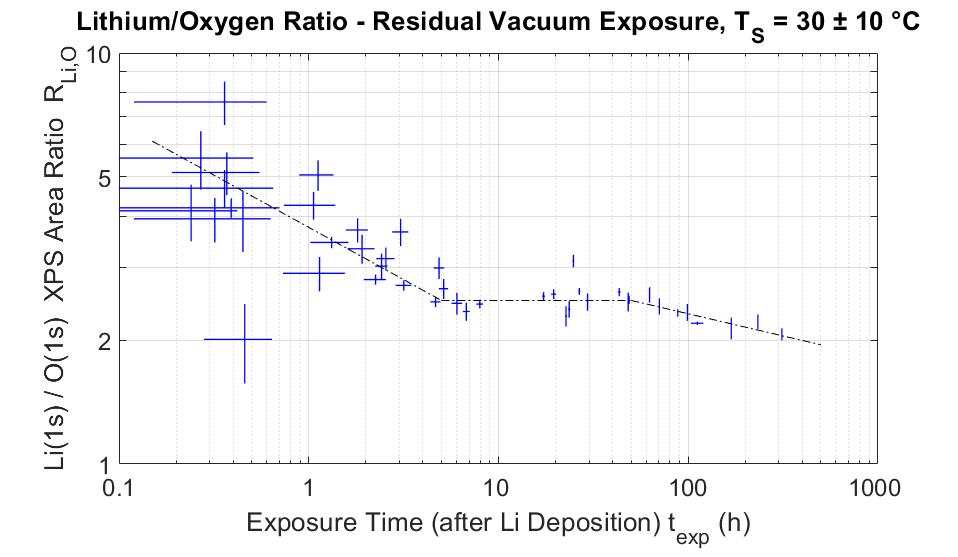
\includegraphics[width=3.37in,keepaspectratio]{Ratio}%
%\caption{Ratio of $Li(1s)$ to $O(1s)$ signal as a function of exposure to LTX %residual vacuum conditions \cite{bob-lucia}}
%\end{figure}

Temporal evolution of lithium and oxygen concentrations were also tracked using MAPP. It was observed that the Li(1s)/O(1s) ratio decreased, until it saturated the XPS probe depth, within 5 hrs \cite{lucia-thesis,lucia-paper}. Beyond that, there was no observable change in the elemental concentration until 100 hrs, after which the Li(1s)/O(1s) ratio began to decrease slowly. The saturation of the ratio of lithium to oxygen to about $2$ was attributed to the growth of $Li_2O$ on freshly deposited lithium in the presence of residual water vapor, consistent with laboratory experiments \cite{50,51}.  Specifically, below 100 $L$ (or Langmuirs, where; $1 L = 10^{-6}Torr-sec$) of $H_2O$ exposure, $Li_2O$ forms preferentially on a clean lithium surface, while at higher exposures there is a transition to $LiOH$ formation. For LTX-relevant water partial pressures, $P_{H_2O}$, 100 $L$ is equivalent 14 hrs of exposure to residual vacuum. It was also observed that the presence of the oxide did not affect plasma performance; LTX continued to get high plasma currents until 40 days after lithium deposition. High plasma performance in the absence of elemental lithium was a surprising result \cite{bob-lucia}. 

An explanation of the oxide growth can be provided by the metal oxide growth kinetics model  \cite{53}, which states that, in general the oxide growth kinetics can be modelled by an advection-diffusion equation. At the onset, the oxide growth is driven by advection; a potential develops across the oxide film that drives the metal ions to the gas-oxide interface and oxygen ions to the metal-oxide interface. As the oxide grows in thickness, the potential across the film is shielded by free electrons and eventually, when the oxide grows thick enough, further growth is dominated by Fickian diffusion. The flux of $H_2O$ molecules impinging onto the surface, for $P_{H_2O}$ in LTX after lithium deposition, is $\Gamma_{H_2O} = 5.6 \times 10^{15} m^{-2}sec^{-1}$. Assuming a sticking co-efficient\cite{51} of S = 1, with this flux it would take 13 min for a monolayer of oxide to form. Since the Li(1s)/O(1s) ratio saturates to $\sim$ 2 after 5 hr \cite{lucia-thesis,lucia-paper}, we assume that the oxide layer took 5 hrs to grow 3 nm in thickness, because 3 nm is the approximate XPS probe depth for MAPP. The metal oxide growth kinetics model then dictates an oxide growth rate of 7.2 $\mathring{A}/hr$ at the onset and 5.5 $\mathring{A}/hr$ at the XPS probe depth in the thin film limit \cite{thin-film}. Note that the oxide growth rate would continue to decrease slowly as the film thickness increased. At the oxide growth rate of 5.5 $\mathring{A}/hr$, a 100 nm coating would take 180 hr to fully oxidize, which is close to the 100 hr period for which there was no observable change in the Li(1s)/O(1s) ratios. \cite{lucia-thesis,lucia-paper} Therefore, it was concluded that lithium coatings on LTX change over a timescale of hours. 

Immediately after the plasma extinguishes in LTX, the Fast Ion Gauge (FIG) shows a 60\% reduction in $H_2$ inventory compared to calibration shots where a plasma was not initiated. Over longer timescales, however, the $H_2$ reading in the Residual Gas Analyzer (RGA) for shots when a plasma was initiated exceeds the recorded measurement for the calibrated gas puffs. This leads to the conclusion that while a significant portion of hydrogen is retained during a plasma, the hydrogen out-gasses over time scales much longer than the plasma duration \cite{bob-lucia,boyle-prl}. With 60\% of the incoming hydrogen ions retained, for a lithium coating of 100 nm and LTX relevant fluence, the Li coating would saturate with hydrogen in \textless 10 shots (assuming Li:H = 1:1). However, this was not the case and plasma performance did not decay after a few of shots, rather after 40 days and close to one hundred shots. This leads to the conclusion that hydrogen is retained by lithium coated PFCs in LTX such that it is free to diffuse out between shots.

\section{Description of Apparatus}

In the previous campaign, LTX (for the current campaign the machine is referred to as LTX-$\beta$) operated with a toroidal field $\sim$ 1.7 $kG$, $I_p$ \textless $80 kA$ and a shot duration $\tau_{discharge}$ \textless $25 msec$. LTX-$\beta$ can achieve double the field and plasma current and close to double the discharge duration with neutral beam fueling. To further study the effect of lithium PFCs on plasma performance in LTX-$\beta$, we propose a Sample Exposure Probe (SEP).

\begin{figure}%
\centering
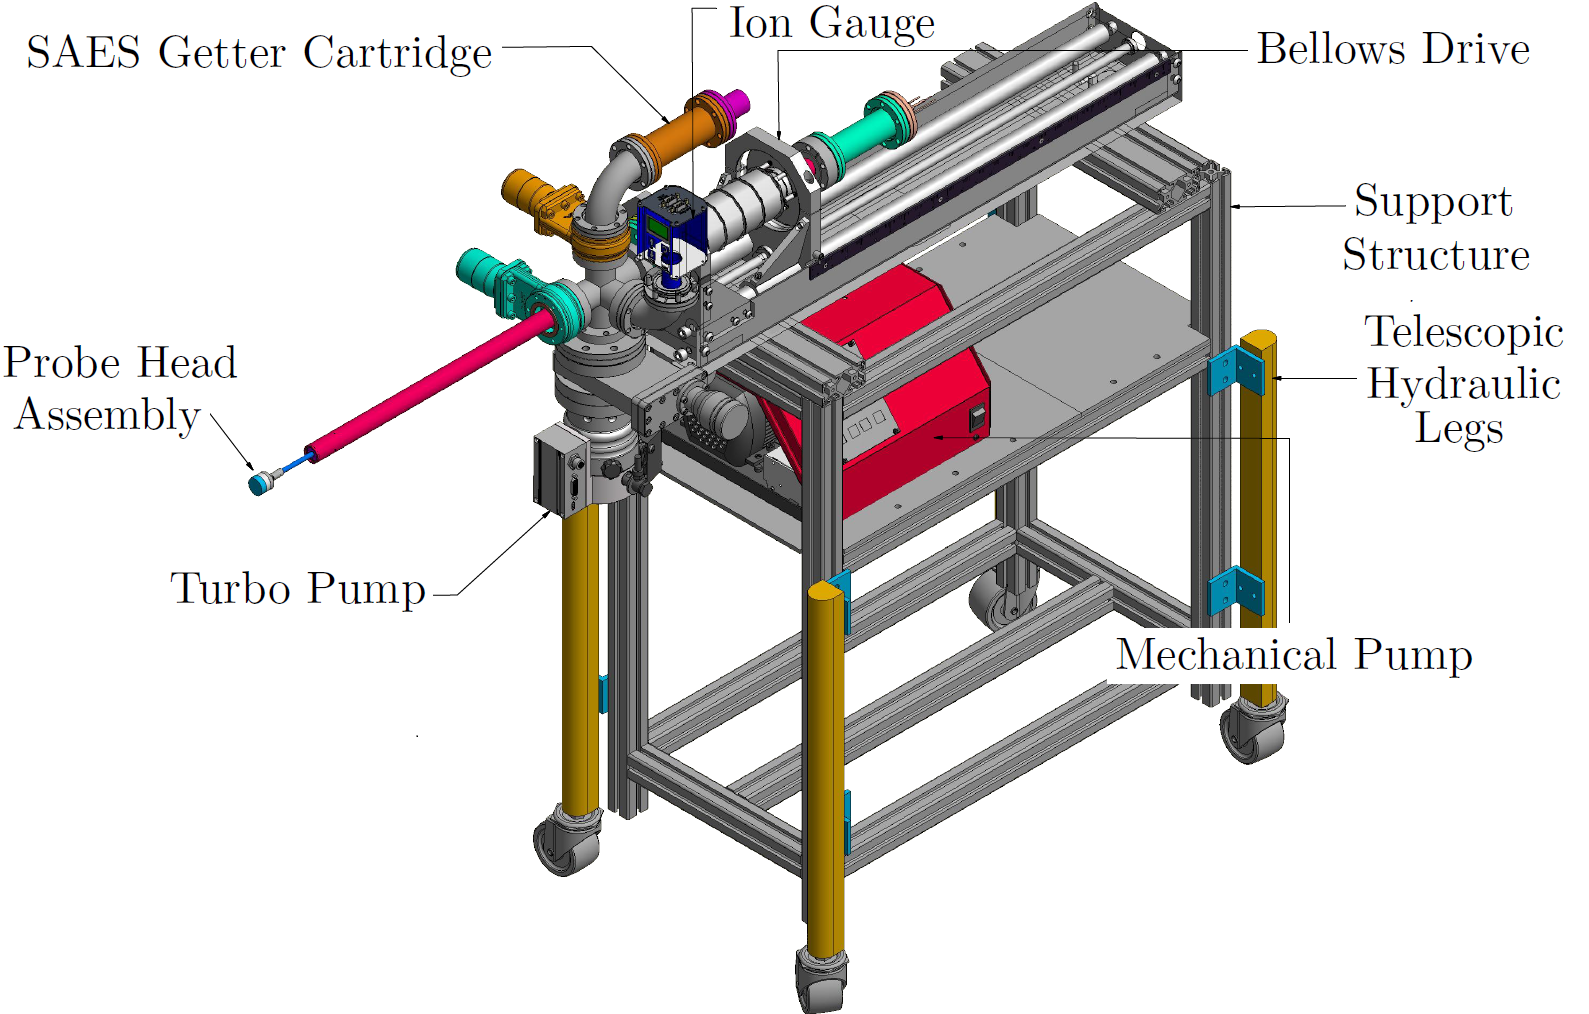
\includegraphics[width=3.37in,keepaspectratio]{SEP_Annotated}%
\caption{Isometric view of the Sample Exposure Probe Assembly}
\end{figure}

The SEP, figure 1, features a SS-304 probe head with a button heater to heat the probe head for Temperature Programmed Desorption (TPD) studies and to mimic LTX-$\beta$ shells in high temperature operations, a thermocouple inserted in the back of the sample head to measure heat flux from the plasma during exposure and to monitor the temperature during TPD. Pumping on the SEP is provided by a 67 $L/sec$ turbomolecular pump and a 100 $L/sec$ non evaporable getter pump. The assembly is mounted in a bellows drive and the drive rests on a 80-20 support structure with telescopic hydraulic legs to facilitate mounting on LTX-$\beta$ and the PHI. The PHI is a UHV (Ultra-High Vacuum) chamber in the Surface Science and Technology Laboratory (SS\&TL). PHI is equipped for XPS, TPD, Ion Scaterring Spectroscopy (ISS) and Sputter Depth Profiling. The PHI has an ultimate base pressure of $2 \times 10^{-10} Torr$; pumping is provided by a 120 $L/sec$ refurbished ion pump, a 170 $L/sec$ turbomolecular pump, a 1000 $L/sec$ titanium getter and a 30 $L/sec$ trubomolecular pump for differentially pumping the ion source. The SEP has an ultimate base pressure of $1.6 \times 10^{-9} Torr$; the base pressure of LTX-$\beta$ after lithium evaporations has been observed to be $6 \times 10^{-8} Torr$. The general idea of the setup is that in-vacuo analysis can be performed on LTX-$\beta$ PFCs by moving samples in-vacuo, under better vacuum conditions to a high resolution system that is nearby. In doing so, design constraints that are imposed on the analysis station, were it built to be in the test cell of the  tokamak are eliminated, enabling analysis with systems that posses higher resolution and better signal to noise ratios. Better vacuum conditions during transfer and analysis reduce the rate of sample contamination and therefore, provide adequate time required for physical transfer of the probe, its analysis and return to the tokamak. 

\begin{figure}%
\centering
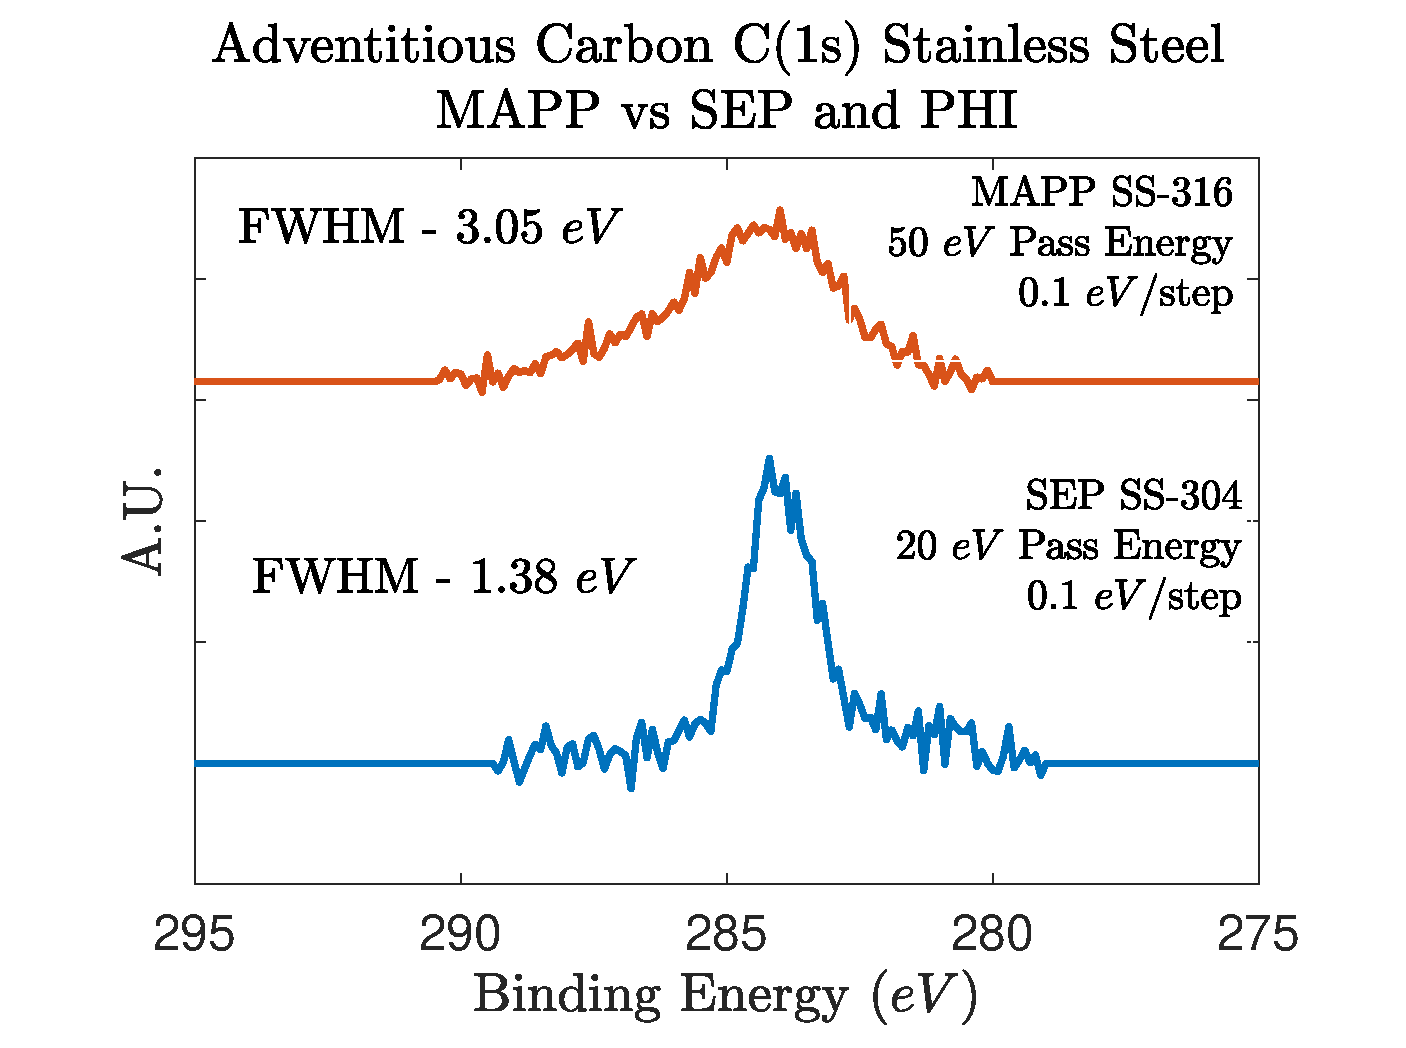
\includegraphics[width=3.37in,keepaspectratio]{C1sMAPP_Comparr_20eV}%
\caption{Adventitious Carbon C(1s) peak on MAPP and SEP}
\end{figure}

\section{Results and Discussion}

Better resolution and signal to noise ratio (SNR) on XPS scans is a key tool to understand how surfaces change in a tokamak and consequently in understanding how they impact plasma performance. Initial XPS scans using the SEP on the PHI show both improved resolution and remarkably better signal to noise ratio. An example of this improvement is shown in figure 2, the two scans belong to the adventitious carbon $C(1s)$ peak on the stainless steel probe head of MAPP and SEP respectively. The scans show a reduction in full width at half max (FWHM) by a factor of 2.2. SNR was measured for both peaks using a commonly used expression for XPS \cite{xps_snr} to be 13.5 for the MAPP peak and 23 for the SEP using PHI. This is attributed to the higher intensity of the X-Ray source on the PHI and a smaller distance from the probehead. The $C(1s)$ peak shown in figure 2, blue (bottom) trace, at $50 eV$ pass energy shows FWHM of $1.8eV$ and an SNR of 64. 

\begin{figure}%
\centering
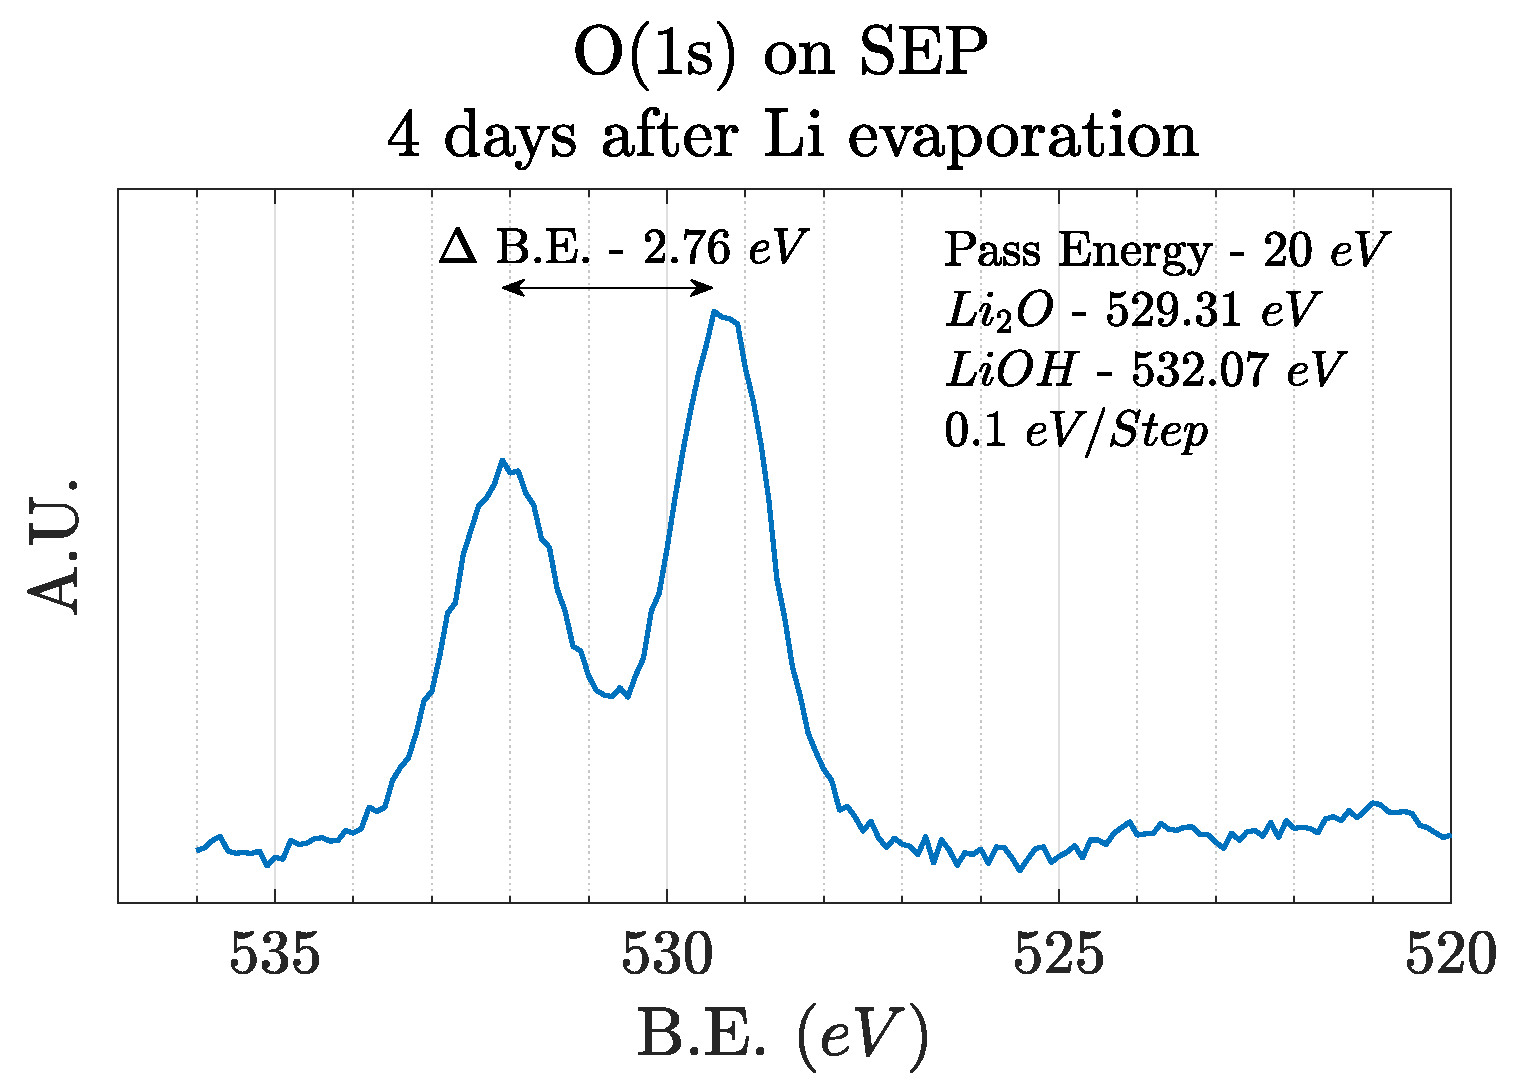
\includegraphics[width=3.37in,keepaspectratio]{O1s_20eV}%
\caption{O(1s) narrow scan of the SEP }
\end{figure}

An example of how improved resolution on XPS scans is helpful in identifying species on the surface is shown in figure 3. It was hypothesized by the previous analysis that $LiOH$ grows on the surface of Li deposited on SS shells of LTX over longer time scales (read hours and beyond), but MAPP did not have the requisite resolution to confirm this. Figure 3 shows a narrow $O(1s)$ scan of the SEP probe head. The scan was taken 4 days after fresh lithium was deposited on the LTX-$\beta$ shells. SEP was docked LTX-$\beta$, and the probe head was made flush with the shells during the Li deposition and subsequent plasma and residual vacuum exposure. The narrow $O(1s)$ scans show two distinct features, the difference in binding energy of the two features are consistent with reported difference between $Li_2O$ and $LiOH$ \cite{o1s_delta}. 

\begin{figure}%
\centering
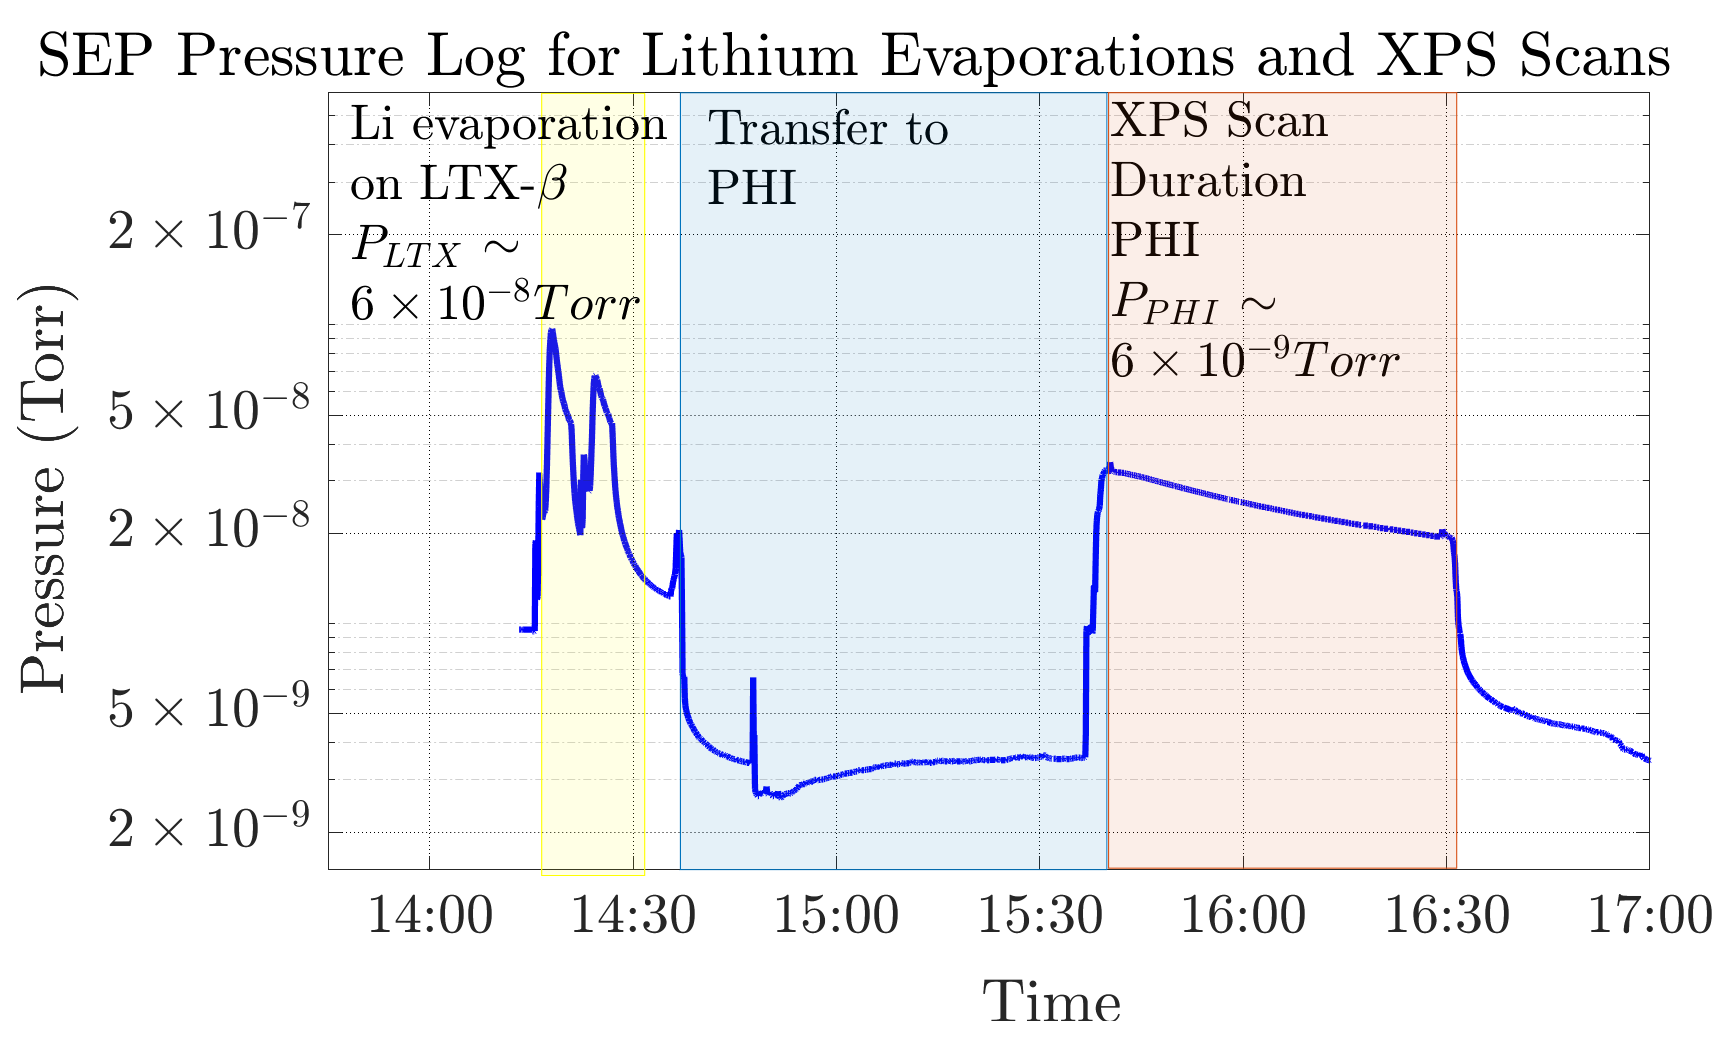
\includegraphics[width=3.37in,keepaspectratio]{04012019_Transferlog}%
\caption{Pressure log from the SEP Ion gauge for transfer from LTX-$\beta$ to PHI, yellow region shows lithium evaporation on the vessel walls, blue region shows SEP pressure during transfer and yellow region for the duration of XPS scans.}
\end{figure}

Because of decent vacuum conditions in LTX-$\beta$, during transfer and in the PHI, it is also possible to probe the surface using XPS at time scales comparable to MAPP. Large error bars at shorter time scales exist in MAPP data because MAPP took time to collect counting statistics to quantify elemental composition. A typical MAPP scan took 45 minutes to take a survey and a few narrow scans of the elements of choice at pressure comparable to LTX. The SEP including transfer to PHI takes 2 hours. However, during transfer and XPS scans, the pressure is maintained between $2-7 \times 10^{-9} Torr$, figure 4. This is an order of magnitude lower than LTX-$\beta$ base pressure. The changes to a lithium surface, therefore, take longer. This is illustrated by the fact that MAPP measured the elemental composition of freshly deposited Li in LTX to be within 70-80 \%. The SEP with PHI pegs the same number at 77.4 $\pm$ 4.4 \% uncorrected (like MAPP) for analyzer transmission function and escape depth.

\begin{acknowledgments}
This work was supported by the US. D.O.E. contract DE-AC05-00OR22725 and DE-AC02-09CH11466. BEK acknowledges support of this work by the U.S. Department of Energy, Office of Science/Fusion Energy Sciences under Award Number DE-SC0012890.

\end{acknowledgments}

%\nocite{*}
\bibliographystyle{aipauth4-1}
\bibliography{references}% Produces the bibliography via BibTeX.

\end{document}
%
% ****** End of file aipsamp.tex ******